\chapter{Компьютерное моделирование гранулярной системы методом дискретных элементов}
\label{cha:research}

Теперь перейдем к проверке построенной нами теоретической модели с помощью компьютерной симуляции рассматриваемой нами системы.
Для этого мы построили компьютерную модель анализируемой нами системы. Мы использовали т.н. \emph{метод дискретных элементов},
где вся система рассматривая как состоящая из множества независимых элементов, динамика каждой из которых рассчитывается 
в зависимости от окружающих факторов в каждый момент времени. В общем случае разделяют два типа подобных симуляций,
это т.н. \emph{движимые событием (event driven)} и \emph{движимые силой (force driven)}. В первом случае, мы полагаем что
вся механика столкновений нам известна, и что зная начальные значения динамических параметров при столкновении, мы можем 
рассчитать сразу же и конечные значения. Таким образом, нам только остается точно определить время столкновения, а вся
динамика системы между столкновениями может считаться простым линейным и равномерным движением, и может быть опущена из рассмотрения.
Преимущества данного метода в том, что шаг по времени эволюции системы зависит от состояния системы, и если мы рассматриваем
разряженную систему, то можно существенно увеличить скорость симуляции. Однако данный метод не подходит для плотных газов,
так как в данном случае скорость симуляции будет стремиться к нулю. В этом случае можно применять метод движимый силой, 
который мы и применяли в данной работе. В этом случае мы фиксируем шаг по времени, желательно соблюдая условие $\Delta t\leq t_{coll}$,
т.е. шаг по времени должен быть не больше $10\%$ от времени столкновения. На каждом шаге симуляции, рассчитываются результирующие 
силы действующие на каждую частицу системы, или на каждый дискретный элемент. В итоге, зная результирующую силу действующую на 
элемент, решая уравнения движения, получаем состояние всей системы в последующий шаг по времени. В нашем случае, все силы,
действующие на элемент, являются контактными, и появляются только при непосредственном контакте элементов друг с другом.
Мы рассматриваем сухой гранулярный газ, без адгезивных поверхностных сил, и в итоге, имеем дело с двумя типами сил 
\cite{Salo:2010icarus_N_body,Schaefer:1996jphys_force_schemes,Cuendet:2007jchem_md_simul,Lois:2007pre_shear_flow,
Brilliantov:2007pre_coll_dyn,Brilliantov:2007pre_coll_adh,Quinn:2010astro_hill_simplectic}. 
Первый тип,
эластичное или упругое взаимодействие двух сферических тел, задается как сила Герца:
\begin{equation}
  F_H(x) = \frac{\sqrt{\sigma_{eff}}}{D}\cdot x^{3/2}\;,
\end{equation}
где
\begin{equation}
  \begin{split}
    x &= \sigma_i + \sigma_j - \vert \br_i-\br_j\vert\;,\\
    D &= \frac{3}{2}\cdot\frac{1-\nu^2}{Y}\;,\\
    \sigma_{eff} &= \frac{\sigma_i\sigma_j}{\sigma_i+\sigma_j}\;,
  \end{split}
\end{equation}
где $\br_i,\;\br_j$ -- координаты центров сталкивающихся элементов. Данная сила является полностью упругой и не приводит к диссипации.
Для учета диссипативных свойств элементов, необходимо ввести дополнительную силу вязкого трения. 

\begin{equation}
  F_{dis}(x,\;\dot{x}) = \frac{3Ax^2}{DR_{eff}}\cdot\dot{x}\;,
\end{equation}
где $\dot{x}$ -- скорость сближения элементов, $A$ -- коэффициент диссипации. Следует отметить, что $F_H$ всегда направлена
от точки столкновения наружу через центра элемента, тогда как $F_{dis}$ всегда направлена против направления движения элемента.
Мы рассмотрели контактные силы. Теперь рассмотрим гравитационные силы центральной, действующие на каждый элемент системы. 
В локальной системе координат, вращающейся вокруг центра планеты с орбитальной частотой $\Omega$, динамика системы 
определяется уравнениями Хилла:
\begin{equation}
  \begin{split}
    &\ddot{x} - 2\Omega\dot{y}+\left(\Omega_r^2-4\Omega^2\right)x = F_x\;,\\
    &\ddot{y} + 2\Omega\dot{x} = F_y\;,\\
    &\ddot{z} + \Omega_z^2z = F_z\;,
  \end{split}
\end{equation}
где $F_x,\;F_y,\;F_z$ -- компоненты контактных сил рассмотренных выше. В нашем случае мы рассматриваем двумерную систему, а также 
эпициклическая $\Omega_r$ и вертикальная $\Omega_z$ частоты равны $\Omega$. Таким образом, мы приходим к следующим уравнениям:
\begin{equation}
  \begin{split}
    &\ddot{x}-2\Omega\dot{y}-\frac{3}{2}\Omega x = F_x\;,\\
    &\ddot{y}+2\Omega\dot{x} = F_y\;. 
  \end{split}
\end{equation}

В нашей симуляции рассматривалась система из $25000$ частиц, по $5000$ в каждой из подсистем (Рис.~\ref{fig:md_sim}).
В начале симуляции, все подсистемы имеют одинаковые энергии, однако с течением времени их энергии расходятся, из-за 
различного количества диссипируемой энергии. Чем больше масса составляющих частиц подсистемы, тем меньше ее диссипация
за счет столкновений, и соответственно тем больше ее энергия относительно других подсистем, с меньшими массами составляющих частиц 
(Рис.~\ref{fig:energy_evo}).

\begin{figure}[ht]
  \centering
  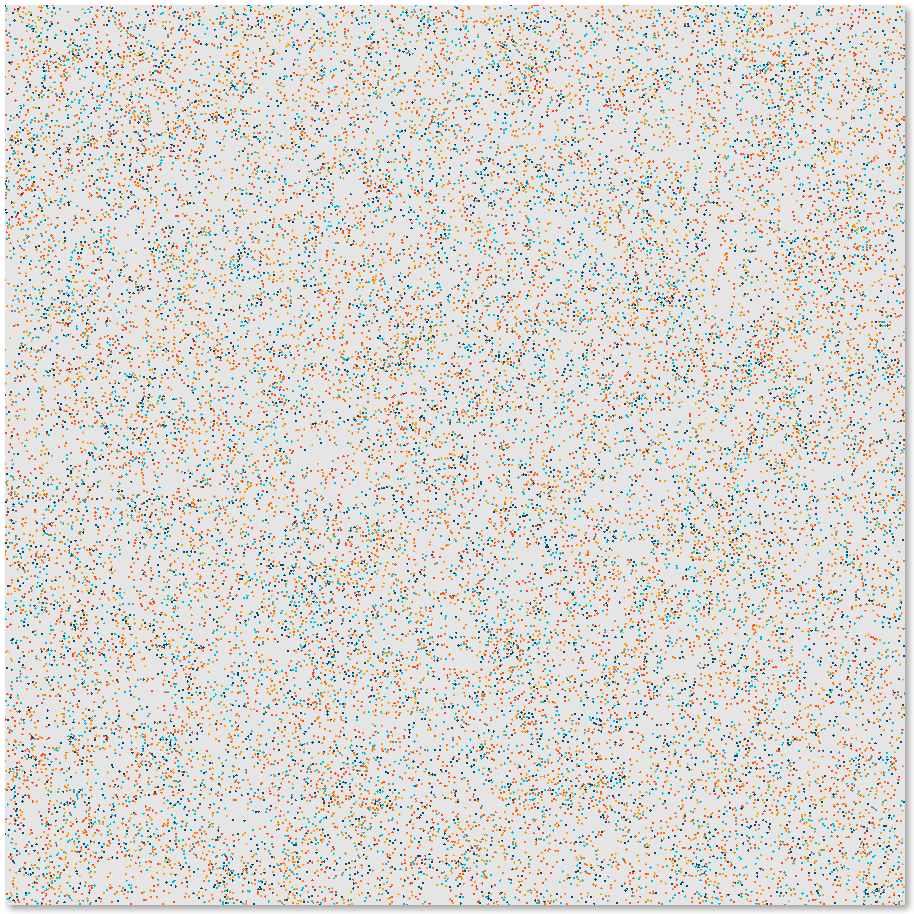
\includegraphics[width=0.7\textwidth]{figures/MD_sim_1.png}
  \caption{Симуляция гранулярной системы из $25000$ частиц. Различными цветами обозначены отдельные подсистемы,
  каждая из которых состоит из $5000$ частиц.}
  \label{fig:md_sim}
\end{figure}

\begin{figure}[ht]
  \centering
  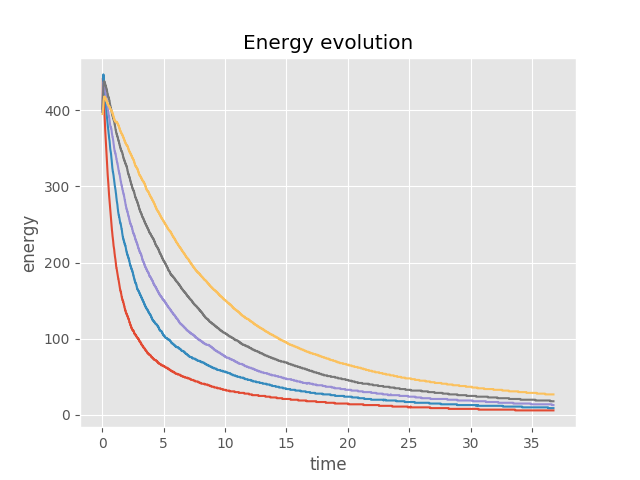
\includegraphics[width=0.7\textwidth]{figures/energy_evo.png}
  \caption{Эволюция энергии системы. Все подсистемы начинают свою эволюцию с одинаковым значением энергии,
  однако с течением времени их энергии расходятся. Чем больше масса частиц подсистемы, тем больше ее энергия.}
  \label{fig:energy_evo}
\end{figure}